% Options for packages loaded elsewhere
\PassOptionsToPackage{unicode}{hyperref}
\PassOptionsToPackage{hyphens}{url}
%
\documentclass[
]{book}
\usepackage{amsmath,amssymb}
\usepackage{lmodern}
\usepackage{iftex}
\ifPDFTeX
  \usepackage[T1]{fontenc}
  \usepackage[utf8]{inputenc}
  \usepackage{textcomp} % provide euro and other symbols
\else % if luatex or xetex
  \usepackage{unicode-math}
  \defaultfontfeatures{Scale=MatchLowercase}
  \defaultfontfeatures[\rmfamily]{Ligatures=TeX,Scale=1}
\fi
% Use upquote if available, for straight quotes in verbatim environments
\IfFileExists{upquote.sty}{\usepackage{upquote}}{}
\IfFileExists{microtype.sty}{% use microtype if available
  \usepackage[]{microtype}
  \UseMicrotypeSet[protrusion]{basicmath} % disable protrusion for tt fonts
}{}
\makeatletter
\@ifundefined{KOMAClassName}{% if non-KOMA class
  \IfFileExists{parskip.sty}{%
    \usepackage{parskip}
  }{% else
    \setlength{\parindent}{0pt}
    \setlength{\parskip}{6pt plus 2pt minus 1pt}}
}{% if KOMA class
  \KOMAoptions{parskip=half}}
\makeatother
\usepackage{xcolor}
\usepackage{longtable,booktabs,array}
\usepackage{calc} % for calculating minipage widths
% Correct order of tables after \paragraph or \subparagraph
\usepackage{etoolbox}
\makeatletter
\patchcmd\longtable{\par}{\if@noskipsec\mbox{}\fi\par}{}{}
\makeatother
% Allow footnotes in longtable head/foot
\IfFileExists{footnotehyper.sty}{\usepackage{footnotehyper}}{\usepackage{footnote}}
\makesavenoteenv{longtable}
\usepackage{graphicx}
\makeatletter
\def\maxwidth{\ifdim\Gin@nat@width>\linewidth\linewidth\else\Gin@nat@width\fi}
\def\maxheight{\ifdim\Gin@nat@height>\textheight\textheight\else\Gin@nat@height\fi}
\makeatother
% Scale images if necessary, so that they will not overflow the page
% margins by default, and it is still possible to overwrite the defaults
% using explicit options in \includegraphics[width, height, ...]{}
\setkeys{Gin}{width=\maxwidth,height=\maxheight,keepaspectratio}
% Set default figure placement to htbp
\makeatletter
\def\fps@figure{htbp}
\makeatother
\setlength{\emergencystretch}{3em} % prevent overfull lines
\providecommand{\tightlist}{%
  \setlength{\itemsep}{0pt}\setlength{\parskip}{0pt}}
\setcounter{secnumdepth}{5}
\usepackage{booktabs}
\usepackage{amsthm}
\makeatletter
\def\thm@space@setup{%
  \thm@preskip=8pt plus 2pt minus 4pt
  \thm@postskip=\thm@preskip
}
\makeatother
\usepackage{booktabs}
\usepackage{longtable}
\usepackage{array}
\usepackage{multirow}
\usepackage{wrapfig}
\usepackage{float}
\usepackage{colortbl}
\usepackage{pdflscape}
\usepackage{tabu}
\usepackage{threeparttable}
\usepackage{threeparttablex}
\usepackage[normalem]{ulem}
\usepackage{makecell}
\usepackage{xcolor}
\ifLuaTeX
  \usepackage{selnolig}  % disable illegal ligatures
\fi
\usepackage[]{natbib}
\bibliographystyle{apalike}
\IfFileExists{bookmark.sty}{\usepackage{bookmark}}{\usepackage{hyperref}}
\IfFileExists{xurl.sty}{\usepackage{xurl}}{} % add URL line breaks if available
\urlstyle{same} % disable monospaced font for URLs
\hypersetup{
  pdftitle={Center for Conservation Biology \textbar{} UC Riverside},
  pdfauthor={Lynn Sweet \textbar{} Principal Investigator, Assistant Research Ecologist; Julia Parish \textbar{} Data Science Intern},
  hidelinks,
  pdfcreator={LaTeX via pandoc}}

\title{Center for Conservation Biology \textbar{} UC Riverside}
\usepackage{etoolbox}
\makeatletter
\providecommand{\subtitle}[1]{% add subtitle to \maketitle
  \apptocmd{\@title}{\par {\large #1 \par}}{}{}
}
\makeatother
\subtitle{Administration Guide}
\author{Lynn Sweet \textbar{} Principal Investigator, Assistant Research Ecologist \and Julia Parish \textbar{} Data Science Intern}
\date{2022-07-22}

\begin{document}
\maketitle

{
\setcounter{tocdepth}{1}
\tableofcontents
}
\hypertarget{informational-resource-for-ccb-faculty-staff}{%
\chapter*{Informational Resource for CCB Faculty \& Staff}\label{informational-resource-for-ccb-faculty-staff}}
\addcontentsline{toc}{chapter}{Informational Resource for CCB Faculty \& Staff}

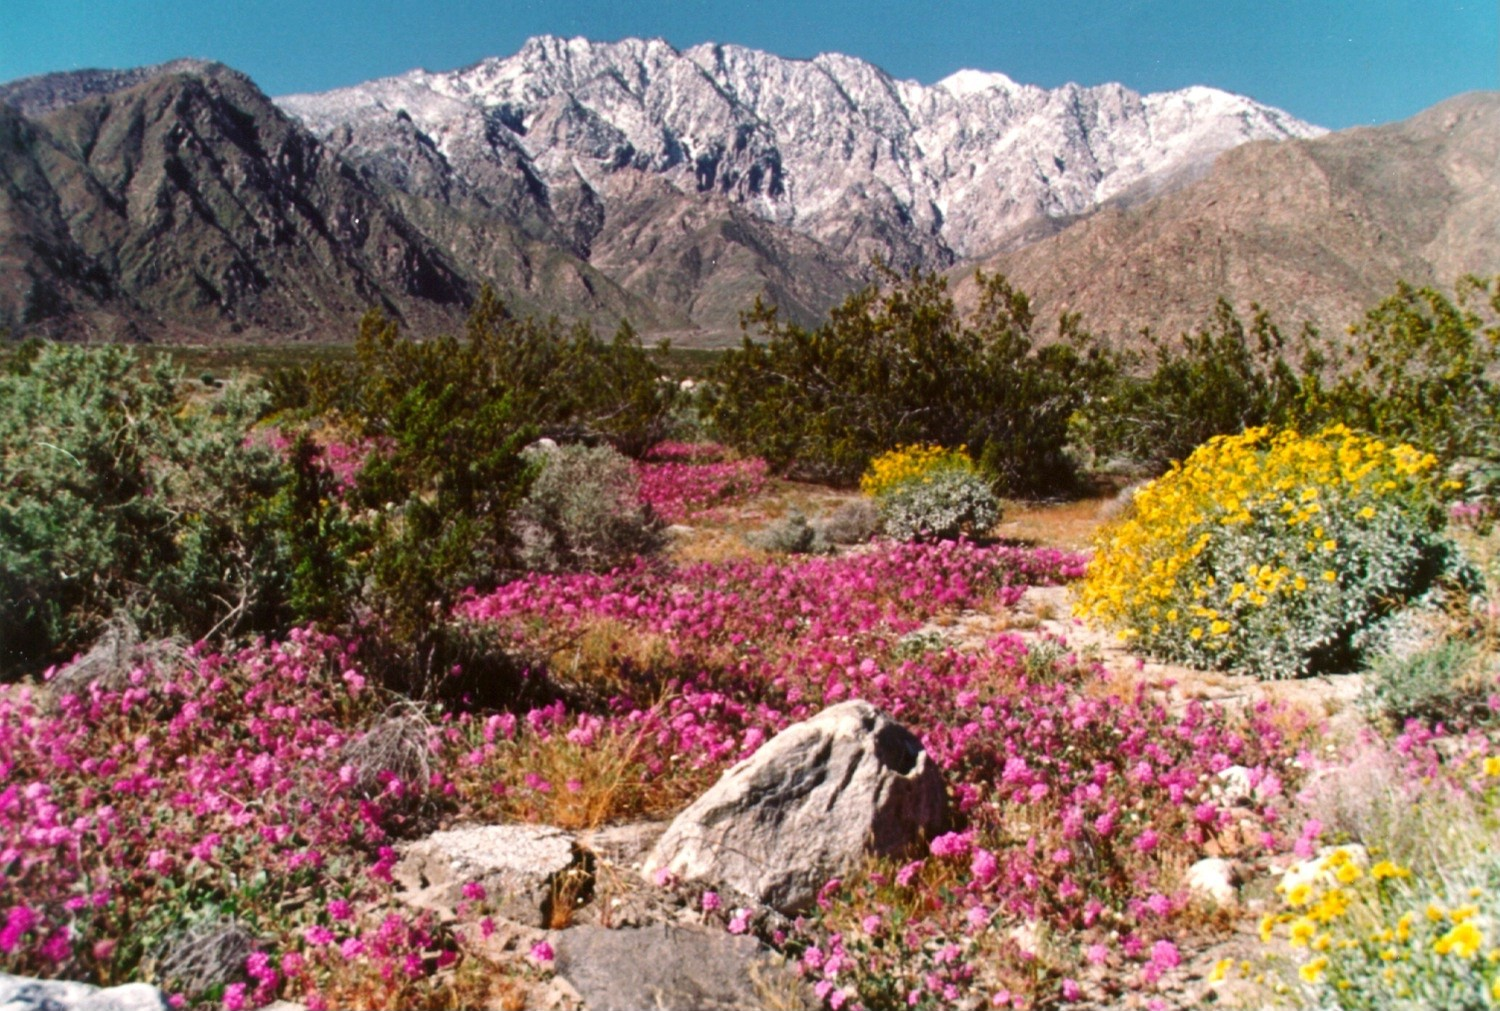
\includegraphics[width=20.83in]{images/cvmc_billhavert}

Chino Canyon Wildflowers, Coachella Valley, California.
\textbf{Image Credit:} Coachella Valley Mountains Conservancy: \emph{Bill Havert}

\begin{center}
\includegraphics[width=12.85in]{images/ucrccb} \end{center}

\hypertarget{intro}{%
\chapter{Introduction}\label{intro}}

\hypertarget{bookdown}{%
\chapter{Bookdown Guide}\label{bookdown}}

The first step to edit and add to this bookdown is to install the \textbf{bookdown} package from CRAN or Github:

\hypertarget{primary-reference-resources}{%
\section{Primary Reference Resources}\label{primary-reference-resources}}

Here is a list of resources to learn how to use and edit in bookdown

\begin{itemize}
\tightlist
\item
  \href{https://bookdown.org/}{Bookdown Package Documentation}
\item
  \href{https://bookdown.org/yihui/bookdown/}{Authoring Books with R Markdown}
\item
  \href{https://bookdown.org/yihui/rmarkdown-cookbook/}{R Markdown Cookbook}
\item
  \href{https://bookdown.org/yihui/rmarkdown/}{R Markdown: The Definitive Guide}
\end{itemize}

\hypertarget{formatting}{%
\section{Formatting}\label{formatting}}

You can use anything that Pandoc's Markdown supports, e.g., a math equation \(a^2 + b^2 = c^2\).

Remember each Rmd file contains one and only one chapter, and \textbf{a chapter} is defined by the first-level heading \texttt{\#}.

You can label chapter and section titles using \texttt{\{\#label\}} after them, e.g., we can reference Chapter \ref{intro}. If you do not manually label them, there will be automatic labels anyway, e.g., Chapter \ref{methods}.

Figures and tables with captions will be placed in \texttt{figure} and \texttt{table} environments, respectively.

\begin{figure}

{\centering 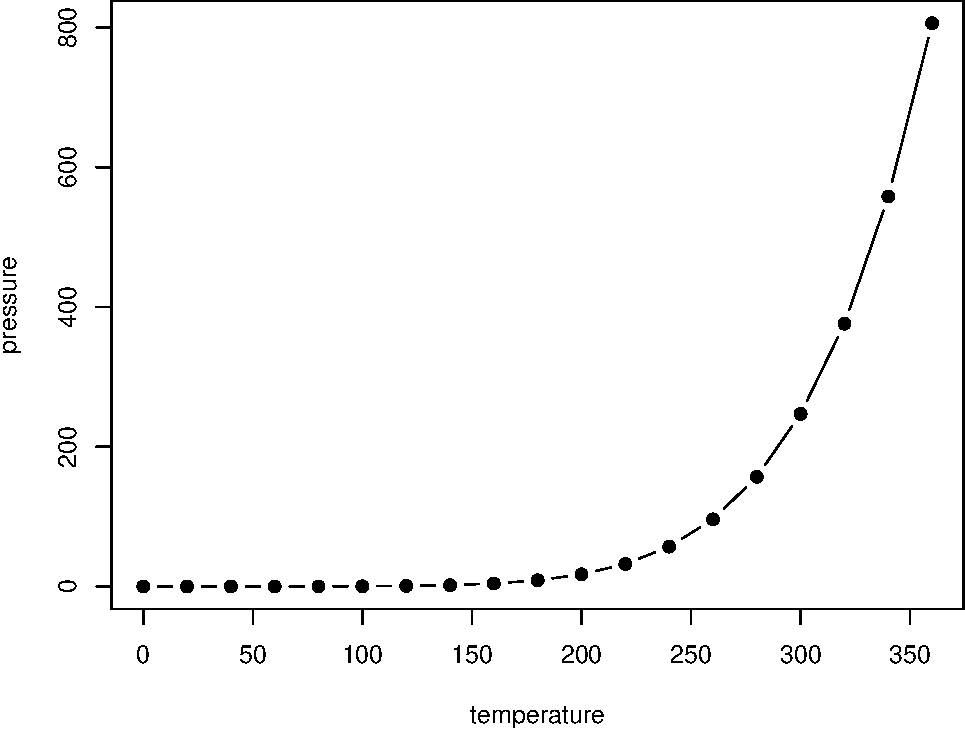
\includegraphics[width=0.8\linewidth]{bookdown-demo_files/figure-latex/nice-fig-1} 

}

\caption{Here is a nice figure!}\label{fig:nice-fig}
\end{figure}

Reference a figure by its code chunk label with the \texttt{fig:} prefix, e.g., see Figure \ref{fig:nice-fig}. Similarly, you can reference tables generated from \texttt{knitr::kable()}, e.g., see Table \ref{tab:nice-tab}.

\begin{table}

\caption{\label{tab:nice-tab}Here is a nice table!}
\centering
\begin{tabular}[t]{rrrrl}
\toprule
Sepal.Length & Sepal.Width & Petal.Length & Petal.Width & Species\\
\midrule
5.1 & 3.5 & 1.4 & 0.2 & setosa\\
4.9 & 3.0 & 1.4 & 0.2 & setosa\\
4.7 & 3.2 & 1.3 & 0.2 & setosa\\
4.6 & 3.1 & 1.5 & 0.2 & setosa\\
5.0 & 3.6 & 1.4 & 0.2 & setosa\\
\addlinespace
5.4 & 3.9 & 1.7 & 0.4 & setosa\\
4.6 & 3.4 & 1.4 & 0.3 & setosa\\
5.0 & 3.4 & 1.5 & 0.2 & setosa\\
4.4 & 2.9 & 1.4 & 0.2 & setosa\\
4.9 & 3.1 & 1.5 & 0.1 & setosa\\
\addlinespace
5.4 & 3.7 & 1.5 & 0.2 & setosa\\
4.8 & 3.4 & 1.6 & 0.2 & setosa\\
4.8 & 3.0 & 1.4 & 0.1 & setosa\\
4.3 & 3.0 & 1.1 & 0.1 & setosa\\
5.8 & 4.0 & 1.2 & 0.2 & setosa\\
\addlinespace
5.7 & 4.4 & 1.5 & 0.4 & setosa\\
5.4 & 3.9 & 1.3 & 0.4 & setosa\\
5.1 & 3.5 & 1.4 & 0.3 & setosa\\
5.7 & 3.8 & 1.7 & 0.3 & setosa\\
5.1 & 3.8 & 1.5 & 0.3 & setosa\\
\bottomrule
\end{tabular}
\end{table}

\hypertarget{citations}{%
\section{Citations}\label{citations}}

You can easily write citations using .bib files within this repository formatted using \href{http://www.bibtex.org/}{BibTEX}. For example, the \textbf{bookdown} package \citep{R-bookdown} in this reference book, which was built on top of R Markdown and \textbf{knitr} \citep{xie2015}.

\hypertarget{alt-text-for-accessibility}{%
\section{Alt Text for Accessibility}\label{alt-text-for-accessibility}}

\href{https://www.rstudio.com/blog/knitr-fig-alt/}{Use the knitr package to add alt text to graphics in R Markdown files}

\hypertarget{rendering-bookdown-to-build-publish}{%
\section{Rendering Bookdown to Build \& Publish}\label{rendering-bookdown-to-build-publish}}

In your Console, type either of these commands depending on which type of render you prefer:

\texttt{bookdown::render\_book("index.Rmd",\ "bookdown::gitbook")}
\texttt{bookdown::render\_book("index.Rmd",\ "bookdown::pdf\_book")}

To compile to PDF, you need XeLaTeX. It is recommended to install TinyTeX (which includes XeLaTeX): \url{https://yihui.name/tinytex/}.

  \bibliography{book.bib,packages.bib}

\end{document}
